\chapter{Chemical Equilibrium Is Not Standing Still}

\begin{kaichang}
An unopened bottle of soda sits on the table. Through its wall, everything looks quiet: not a bubble in sight. You unscrew the cap---``Hiss!''---and countless bubbles race upward like children bursting out of a classroom after being cooped up too long.

First, guess the answers to three questions and write them down:

First, before you opened the bottle, were the gas molecules ``crammed inside, holding their breath until you opened the door''?

Second, why does soda left open for a day go ``flat,'' as dull as sugar water? Has all its gas escaped?

Third, put one bottle in the refrigerator and another near a radiator. Which will have more ``kick'' when opened? Why?

By this chapter's end, we will answer using a term you have probably heard but quite possibly misunderstood: \textbf{chemical equilibrium}. Many people think ``equilibrium'' means stopping, no movement, and equal amounts on both sides. Our task is to dismantle these three assumptions one by one.
\end{kaichang}

\section{First, Notice Reversibility}

Almost all the reactions discussed in previous chapters seemed to go ``all the way down a one-way street'': magnesium ribbon burns to magnesium oxide and does not change back by itself (Chapter 26). But nature also has a large class of reactions with \textbf{two-way traffic}: while reactants become products, products also turn back into reactants. These are \textbf{reversible reactions}.

You have already seen signs of reversible processes, even if you did not think of them chemically:

\begin{itemize}[itemsep=2pt]
\item Soda and beer bubble when opened. If gas can come out of water, how did it get in originally? In and out: that is two-way traffic.
\item Add salt to water until no more dissolves, leaving grains on the bottom: Chapter 25 called this ``saturation.'' But does ``no more dissolves'' really mean dissolution has stopped? You will soon find the answer surprising.
\item Mountain climbers become breathless at altitude and recover on returning to the plains. Blood taking up and releasing oxygen is another two-way tug-of-war.
\item Color-changing lipstick kept cold, and heat-sensitive cups that change color when heated, can change back again. These involve another kind of equilibrium, which we will encounter in Chapter 35's coordination chemistry.
\end{itemize}

One more phenomenon deserves a special mention, but \textbf{watch it only on video}: reddish-brown nitrogen dioxide gas sealed in a glass tube becomes noticeably paler in ice water, then darker again in hot water. The changing color shows that two substances inside are interconverting, with temperature reversing the preferred direction. Nitrogen dioxide is toxic. Only a teacher in a fume hood may demonstrate this experiment; \textbf{never try it at home}. Remember the image: change the temperature, and the proportions of two substances in a container change too. Behind those proportions lies this chapter's main character.

\section{Zoom In: Both Directions Run at Once}

Now zoom down to the molecular scale to see what really happens inside a soda bottle.

The soda contains many dissolved carbon dioxide molecules. As Chapter 25 explained, dissolving does not mean disappearing: solute particles spread among solvent particles. Above the liquid and below the cap is a small space also packed with carbon dioxide molecules, at several times the outside pressure. This produces the hiss when you unscrew the cap.

Here is the key picture: \textbf{at every moment, carbon dioxide molecules leap out of the water into the air while others plunge from the air into the water}. Think of a swimming pool, with people constantly diving in and climbing out. Before the bottle is opened, exactly as many dive in as climb out, so the surface conditions---the gas pressure above it and concentration below it---seem perfectly still. It is not that nobody moves, but that \textbf{entry and exit are tied}.

This is the first misconception to dismantle: apparent ``stillness'' is \textbf{dynamic equilibrium} at the particle level. Opposing changes proceed simultaneously at equal rates, canceling macroscopically while remaining bustling microscopically.

In chemical terms, a reversible reaction reaches \textbf{chemical equilibrium} when its forward rate, turning reactants into products, equals its reverse rate, turning products back into reactants. Chapter 29 explained that reaction rates depend on effective collision frequency. As reactants are consumed and their concentrations decrease, the forward reaction slows; as products accumulate, the reverse reaction speeds up. One slows while the other quickens, so their curves must eventually meet: that is equilibrium. Here is a human-made schematic, with unnumbered axes indicating trends and illustrative curves rather than measured data:

\begin{center}
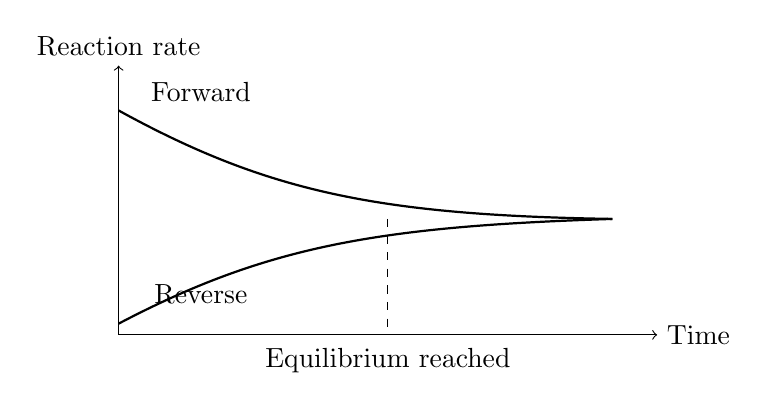
\begin{tikzpicture}[scale=0.95]
\draw[->] (0,0) -- (7.2,0) node[right] {Time};
\draw[->] (0,0) -- (0,3.6) node[above] {Reaction rate};
\draw[thick] (0,3.0) .. controls (2,1.9) and (3.5,1.6) .. (6.6,1.55);
\draw[thick] (0,0.15) .. controls (2,1.2) and (3.5,1.45) .. (6.6,1.55);
\node at (1.1,3.25) {Forward};
\node at (1.1,0.55) {Reverse};
\draw[dashed] (3.6,1.55) -- (3.6,0);
\node at (3.6,-0.35) {Equilibrium reached};
\end{tikzpicture}
\end{center}

Notice that neither line \textbf{falls to zero} after equilibrium. They merely become equal. The reactions keep running, forever, but equally fast in both directions.

\section{Equal Rates Do Not Mean Equal Amounts}

This is the chapter's easiest trap to fall into, and deserves its own section.

In everyday language, ``equilibrium'' suggests ``equal weight on both sides'': a balanced scale has equal weights. Many people casually transfer this image to chemistry: surely reaching equilibrium means equal amounts of reactants and products?

Not at all. What becomes equal is \textbf{the rates in the two directions}, not \textbf{the amounts of the two substances}.

Return to the pool analogy: only when equal numbers dive in and climb out does the number in the pool remain steady. Whether it settles at a hundred swimmers or ten depends on how ``easy'' entering and leaving are. Warm water encourages lingering, so more people are in the pool at equilibrium; icy water makes people reluctant to return after climbing out, so fewer remain. In both cases the inward and outward ``flows'' are equal, yet the ``stock'' inside differs enormously.

Chemistry works the same way. Some reactions reach equilibrium with almost entirely products and only a trace of reactants: we say equilibrium ``lies to the right,'' and the reaction appears to have gone to completion. Others have almost entirely reactants and only traces of products, as though no reaction occurred. Yet given time and a tightly closed lid, both systems sustain two-way reactions at equal rates. What we see as the distinction between ``one-way'' magnesium combustion and ``reversible'' soda degassing is, to a chemist, a difference of countless orders of magnitude in \textbf{how strongly equilibrium favors one side}.

Can we express this preference with a number? Yes: the \textbf{equilibrium constant}.

\begin{qiaoliang}
At equilibrium in a reversible reaction, multiply the product concentrations together and divide by the product of the reactant concentrations, raising each concentration to the power given by its coefficient in the equation. The resulting quotient is \textbf{always constant at the same temperature}. Whether you start with reactants, products, or any mixture, the system eventually adjusts to this number: the equilibrium constant $K$.

The size of $K$ directly indicates which side equilibrium favors:
\begin{itemize}[itemsep=2pt]
\item Very large $K$, such as $10^{15}$: products overwhelmingly dominate at equilibrium and reactants are almost exhausted. The reaction goes ``almost to completion.''
\item Very small $K$, such as $10^{-10}$: reactants overwhelmingly dominate and products appear only in traces. The reaction ``hardly happens.''
\item $K$ near $1$: both sides are comparably strong; neither wipes out the other at equilibrium.
\end{itemize}
One more point must be firmly fixed: $K$ changes only with \textbf{temperature}. Changing concentration or pressure merely makes the system \textbf{reestablish the same $K$ under new conditions}; it cannot alter $K$ itself. A catalyst cannot even touch it: Chapter 30 explained that catalysts only speed the approach to equilibrium, without changing its position.
\end{qiaoliang}

\section{How the System Responds to Disturbance}

Now for the chapter's most useful thought experiment: disturb a system already at equilibrium by adding reactant, compressing a gas, or raising the temperature. What happens?

The system neither passively accepts your action nor completely cancels it. It \textbf{shifts in a direction that weakens the disturbance}, until it again establishes the proportion required by the equilibrium constant. This is \textbf{Le Chatelier's principle}. Consider each case:

\textbf{Changing concentration.} Add reactant to an equilibrium system, and the forward reaction suddenly has more ``raw material.'' More frequent collisions temporarily make it outrun the reverse reaction, converting some added reactant to product until the rates match again. Conversely, \textbf{remove} product by precipitation, outflow, or pumping, and the reverse reaction loses its ``ammunition.'' The forward reaction continues to fill the gap. This principle is immensely valuable in industry, as the ammonia story will soon show.

\textbf{Changing pressure.} This \textbf{works only for gas reactions}, and only when the two sides contain different numbers of gas molecules. Compressing the volume raises pressure, crowds gas molecules together, and increases collision frequency. If one reaction direction reduces the total number of gas molecules, moving that way ``relieves the crowding.'' In ammonia synthesis, for instance, four gas molecules on the left become two on the right, so increased pressure pushes equilibrium rightward. With equal gas molecule counts on both sides, increased pressure treats both equally and equilibrium stays put.

\textbf{Changing temperature.} This is the only disturbance that \textbf{changes $K$ itself}. Heating adds energy: the endothermic direction gets a tailwind, while the exothermic direction is suppressed. Thus heating decreases $K$ for an exothermic reaction and increases it for an endothermic one. The nitrogen dioxide tube becoming paler when cold and darker when hot directly demonstrates temperature rewriting $K$ and shifting equilibrium.

Le Chatelier's principle is quick and intuitive, a useful guide to direction. But remember its limitation, discussed further in the section on boundaries: it tells you \textbf{which way}, never \textbf{how much}.

\section{Symbols Enter the Picture}

Now that we have unpacked the idea, we can write symbols. A reversible reaction uses two opposing half-arrows instead of one single-headed arrow, indicating simultaneous reaction in both directions. Ammonia synthesis is written:

\[\chem{N_2} + \chem{3H_2} \rightleftharpoons \chem{2NH_3}\]

Read it as nitrogen and hydrogen becoming ammonia while ammonia decomposes back into nitrogen and hydrogen. Traffic runs both ways; which direction carries more depends on how far the system currently is from equilibrium.

Carbon dioxide entering and leaving soda is written:

\[\chem{CO_2}\text{(gas)} \rightleftharpoons \chem{CO_2}\text{(dissolved in water)}\]

For the equilibrium constant, use ammonia synthesis as an example: product concentrations go in the numerator, reactant concentrations in the denominator, and coefficients become exponents:

\[K=\frac{[\chem{NH_3}]^{2}}{[\chem{N_2}][\chem{H_2}]^{3}}\]

Square brackets mean ``the concentration of.'' Notice the exponents: ammonia's coefficient is 2, so its concentration is squared; hydrogen's coefficient is 3, so its concentration is cubed. These are not decorative numbers chosen at whim. They arise from particle-collision counting rules, bringing Chapter 29's reasoning into equilibrium. Pure solids and pure liquids, such as the bulk water in a soda bottle, are omitted: their own ``concentrations'' are constant and absorbed into $K$.

\section{How Scientists Know: Food, Explosives, and Equilibrium}

\begin{zhengju}
Early twentieth-century Europe faced a quiet crisis: its population was growing and farmland needed nitrogen fertilizer. Natural nitrate deposits were nearly exhausted, while the air held an abundant supply of potential fertilizer: nitrogen makes up about $78\%$ of air. Unfortunately, its triple bond is too strong (Chapter 18) for plants or people to tackle. Whoever could ``fix'' atmospheric nitrogen as ammonia held the key to food.

Interestingly, Le Chatelier himself, the French chemist who formulated the equilibrium-shift principle, attempted ammonia synthesis in 1901. His principle told him to increase pressure, but air contaminated the experiment, and hydrogen and oxygen exploded under high pressure, nearly killing someone. He abandoned the effort.

The German chemist Haber took up the problem. Rather than charge ahead blindly, he began with \textbf{accounting}: measuring equilibrium constants at different temperatures and pressures. The numbers delivered two pieces of bad news and one of good. First, at room temperature $K$ was pitifully small, placing equilibrium almost entirely on the nitrogen-and-hydrogen side. Second, heating sped the reaction, but because ammonia synthesis is exothermic, it drove $K$ even lower: speed and equilibrium position demanded opposite temperatures. The good news was that pressure could greatly increase the equilibrium proportion of ammonia. Moreover, \textbf{cooling and removing} ammonia and \textbf{recycling} unreacted nitrogen and hydrogen through compression again exploited Le Chatelier's ``remove the product'' strategy, forcing progress cycle after cycle.

In 1909, Haber's apparatus steadily produced ammonia at about 200 atmospheres and $500\,^{\circ}\mathrm{C}$. That temperature was a compromise between ``equilibrium wants cold'' and ``speed wants heat,'' with a catalyst (Chapter 30) addressing the speed shortfall. The engineer Bosch then scaled it into a factory: the Haber--Bosch process still used today. Nitrogen atoms that passed through this pipeline now occur in the proteins of roughly half the world's population.

Remember the other side of the story too: the same ammonia plant can switch production lines to make explosives, and played an inglorious role in both world wars. Scientific principles take no side; people choose the direction. For this chapter, the key is the method. Where did Haber succeed? Not in ``knowing Le Chatelier's principle''---Le Chatelier knew it too---but in \textbf{calculating quantitatively with equilibrium constants}. He determined the exact ammonia fraction at each temperature and pressure, then designed recycling and product removal accordingly. Principles point the direction; numbers determine the plan. Neither works without the other.
\end{zhengju}

\section{Try It: Temperature and Soda Equilibrium}

\textbf{Translator safety note:} The bottle instructions below conflict about whether the warm sample is open. Do not heat a sealed carbonated bottle or use the inconsistent sequence as a protocol; ask a teacher to supply a reviewed comparison. Do not drink experimental samples. See \href{https://institute.acs.org/acs-center/lab-safety/education-training/safer-experiments.html}{ACS guidance on selecting safer activities}.

\begin{shiyan}
\textbf{Materials:} two small soda bottles of the same brand and size (plastic is safer than glass); a refrigerator; a basin of warm water, comfortable to the hand, about $40\,^{\circ}\mathrm{C}$ and never scalding; two identical clear cups; a timer or phone stopwatch.

\textbf{Procedure:}
\begin{enumerate}[itemsep=1pt]
\item Refrigerate one bottle for at least two hours; immerse the other in warm water for the same time (leave it open beside you; do not heat a sealed bottle).
\item Take them out together, quickly unscrew their caps in succession, and immediately pour each into a cup.
\item Observe and record the duration and strength of the opening hiss, the vigor of bubbling in the cups, and how long the foam lasts.
\end{enumerate}

\textbf{What to observe:} which bottle hisses louder? Which cup produces more bubbles, and for longer? After both sit on the table for an hour, has the difference grown or shrunk?

\textbf{Safety:} use \textbf{warm water} only. Never use boiling water, a microwave, or an open flame to heat a sealed carbonated drink: rapidly rising internal pressure could burst the container. Handle gently and do not shake vigorously before opening. Drinking the experimental samples is entirely fine.
\end{shiyan}

You will see that the refrigerated bottle is noticeably ``fizzier'': a longer hiss and denser bubbles. This is temperature shifting equilibrium. Dissolving carbon dioxide in water is exothermic, so cooling pushes this process forward and increases its equilibrium constant, allowing the same bottle to hold more dissolved gas at lower temperature. In the warm-water bottle, much of the gas has already ``climbed ashore'' into the headspace, leaving less in the water. The label ``best served chilled'' has real changes in equilibrium constants behind it.

Make an order-of-magnitude estimate to see how many molecules this equilibrium governs. A \ud{500}{mL} carbonated drink has about \ud{2}{g} to \ud{3}{g} of carbon dioxide forced into it at the factory. Taking \ud{2}{g} and a molar mass of approximately \ud{44}{g/mol} gives $2\div 44\approx 0.045\ \mathrm{mol}$. Multiply by \ud{6.02\times 10^{23}}{} molecules per mole to obtain about $2.7\times 10^{22}$ molecules. In other words, when you unscrew the cap, over two sextillion molecules face a fresh verdict on ``stay or leave,'' decided by that $K$ under the new pressure and temperature.

\section{Equilibrium in Your Body: Carrying Oxygen}

Le Chatelier's principle governs breathing as well as factories. Hemoglobin in blood is a protein that reversibly binds oxygen. Chapter 15 mentioned iron's role in it, and we will return to it among biological macromolecules. Oxygen molecules can ``board'' hemoglobin or ``get off'' again: a textbook reversible process.

In the lungs, oxygen partial pressure in the alveoli is high, equivalent to continually ``adding reactant'' to the equilibrium system. Hemoglobin binds large amounts of oxygen, loading up fully. When blood reaches oxygen-consuming tissues such as muscle and brain, cells have used up oxygen and its concentration is low, equivalent to ``removing product.'' Equilibrium reverses direction and hemoglobin unloads oxygen for the cells. Loading and unloading depend entirely on the same equilibrium automatically shifting gears under different conditions at the two ends, without instructions from the brain.

This explains several familiar phenomena. On first reaching a high plateau, thin air and low oxygen partial pressure prevent hemoglobin from filling up, causing breathlessness and headaches. After a few weeks, the body manufactures more hemoglobin, effectively adding ``carriers'' to the equilibrium system. More oxygen can then be transported in the same low-oxygen environment, and you gradually adapt. Carbon monoxide's danger also involves equilibrium: it binds hemoglobin far more strongly than oxygen, and once seated, is reluctant to give way. From an equilibrium perspective, this blocks oxygen's transport route, so even a small amount in air can be fatal. Keeping ventilation when using a gas water heater is not empty advice: it protects the chemical equilibrium in your blood.

\section{When Does This Model Fail?}

Le Chatelier's principle is useful, but it is \textbf{a directional guide, not a quantitative calculator}. It tells you that pressure increases ammonia, not by what percentage. For numbers, you must calculate using equilibrium constants, as Haber did. More awkwardly, it can sometimes give \textbf{ambiguous or misleading} answers: with simultaneous disturbances, the direction that ``weakens the disturbance'' may be unclear; pressure conditions are largely ineffective for equilibria involving solids and pure liquids; and in systems with several coupled equilibria, such as blood, applying the principle to just one may miss chain effects through the others. Engineers therefore decide using $K$ calculations, not rules of thumb. The challenge at this chapter's end gives a quantitative way to determine direction.

The equilibrium model itself has limits. First, it describes a \textbf{closed system}, one that matter cannot enter or leave. An open soda bottle never reaches true equilibrium because escaping gas molecules do not return. Second, reaching equilibrium \textbf{takes time}: some reactions have enormous equilibrium constants but are so slow that no change appears for tens of thousands of years (Chapter 29). ``What eventually happens'' and ``what is happening now'' require separate accounts. Third, and most profoundly, \textbf{life does not live at equilibrium}. A cell at complete chemical equilibrium is dead: exhausted ATP, flattened concentration gradients, and balanced reaction rates mean no net change remains available to do work. Living cells maintain a \textbf{steady state}, continually taking in matter and energy and expelling waste. They look stable while every molecule flows, like the shape of a fountain rather than the surface of a pond. This thread---life requires being far from equilibrium---will become central to Volume II's discussion of metabolism.

\begin{wuqu}
``When a reaction reaches equilibrium, it stops, and there are equal amounts on both sides.'' Two errors in one sentence, yet this is the most popular version.

Evidence against ``stopping'': put a small salt crystal into \textbf{already saturated} saltwater. If everything had stopped, nothing would happen. But suppose the water already contained dissolved radioactive sodium, the tracer atoms scientists use, almost chemically identical to ordinary sodium but with nuclei that emit detectable signals. Test the crystal a few days later, and it contains radioactivity. There is only one conclusion: the crystal at the bottom is \textbf{continually dissolving}, while dissolved ions are \textbf{continually crystallizing}. Equal rates leave the crystal's mass unchanged, but some of its constituent particles have been replaced. Equilibrium is a tie in exchange, not its termination.

Evidence against ``equal amounts'' runs throughout this chapter. A reaction with an equilibrium constant above $10^{10}$ leaves not even one hundred-millionth of its reactants at equilibrium; one below $10^{-10}$ scarcely produces even traces of products. Both can be perfectly well at equilibrium: equal rates, vastly unequal amounts.
\end{wuqu}

\section{Back to That Bottle of Soda}

Now for the three promised answers.

First, were the molecules ``holding their breath until you opened the door''? No. Dissolution and escape were already tied in the unopened bottle: every second, carbon dioxide molecules emerged from the surface and just as many were pressed back into the water. They neither hold their breath nor wait, but maintain high-pressure equilibrium through dynamic exchange. The cap was not ``blocking'' an intention; it maintained the boundary conditions for that equilibrium.

Second, why does the drink go flat after a day open? On opening, high-pressure carbon dioxide above the liquid disperses into the air, sharply lowering its concentration and almost wiping out the reactants on the ``ashore'' side. Equilibrium receives a strong shove, and the system responds only by weakening that disturbance: dissolved carbon dioxide continually escapes, trying to reestablish the appropriate ratio between the phases. But the bottle is open, and escaping molecules drift away without returning. This is an \textbf{open system}; true equilibrium can never form, so one-way net loss continues until the dissolved gas falls to the very low level corresponding to air. The remaining sugar water has not ``reached equilibrium''; it has given up resisting.

Third, does chilled or warm soda have more kick? The experiment has told you: the cold bottle holds more dissolved gas. Because dissolution is exothermic, low temperature raises the equilibrium constant, letting colder water ``hold down'' more carbon dioxide at the same bottle pressure. In your mouth, body heat warms the soda and shifts equilibrium back, releasing gas. That tingling sensation is the sound of hundreds of quadrillions of molecules collectively ``climbing ashore.''

\section{Deeper Still: Reactions beneath the Surface}

We have told only half the soda story. Not all dissolved carbon dioxide remains simply ``dissolved gas molecules.'' A small fraction truly reacts with water, forming a substance that can donate protons: carbonic acid. This gives soda its mild sourness, makes rain naturally weakly acidic, and dissolves limestone into caves and stalactites over millions of years.

Reversible reactions that ``pass protons back and forth'' form one of chemical equilibrium's largest and most important families. They determine stomach-acid strength, why a sip of vinegar does not acidify your blood, and why shells thin when the ocean absorbs excess carbon dioxide. This family has its own name and accounting scale, and deserves a whole chapter: Chapter 32, the story of acids and bases.

\begin{tiaozhan}
The quantitative version of Le Chatelier's principle takes just one step: substitute \textbf{current} rather than equilibrium concentrations into the equilibrium-constant expression. The result is the \textbf{reaction quotient} $Q$. For ammonia synthesis, $Q=\dfrac{[\chem{NH_3}]^{2}}{[\chem{N_2}][\chem{H_2}]^{3}}$, calculated with the actual concentrations right now.

Then make one comparison:
\begin{itemize}[itemsep=2pt]
\item $Q<K$: products are ``in deficit,'' so the reaction proceeds \textbf{forward} until $Q$ catches $K$;
\item $Q>K$: products are ``over budget,'' so the reaction moves \textbf{in reverse};
\item $Q=K$: equilibrium, with no macroscopic change.
\end{itemize}
Every part of Le Chatelier's principle translates into this comparison. Add reactant, and the denominator grows, $Q$ shrinks, and the reaction goes forward. Remove product, and the numerator shrinks, again lowering $Q$ and favoring forward progress. Compress an ammonia-synthesis mixture, and all concentrations increase by the same factor, but the denominator's total exponent ($1+3=4$) exceeds the numerator's ($2$), so $Q$ again decreases. Pressure shifts equilibrium rightward because of the exponents. Temperature acts separately, directly rewriting $K$ itself. Mastering the comparison of $Q$ and $K$ upgrades Le Chatelier's principle from a mnemonic to an algorithm. You can skip this section without losing the main thread.
\end{tiaozhan}

\section*{Try It Yourself}

\begin{sikaoti}
\item Draw a ``two-box diagram'': left and right boxes represent reactants and products, small dots represent molecules, and two circulating arrows of different thicknesses represent forward and reverse rates. Show a state ``already at equilibrium, but with far more molecules on the right.'' Add a note that this is a human-made representation and the dots' sizes and colors do not show molecules' real appearance.
\item A system is at equilibrium when you suddenly add a large amount of reactant. Sketch reaction rate against time: how do the forward and reverse rates jump at that instant, and how do the curves subsequently meet again? Refer to this chapter's diagram, but show the whole disturbance-and-recovery sequence.
\item Three reactions have equilibrium constants of about $10^{12}$, $1$, and $10^{-8}$ at the same temperature. Without looking anything up, identify the one that goes ``almost to completion,'' the one that ``hardly occurs,'' and the one with evenly matched sides at equilibrium. Then say what happens to each $K$ if all three receive catalysts.
\item Explain using equilibrium shifts why opened soda goes flat faster at room temperature than in a refrigerator. Why does vigorously shaken soda spray when opened? Hint: shaking changes opportunities for gas--liquid contact; first decide whether it changes the rate or the equilibrium position.
\item New arrivals at high altitude breathe rapidly but gradually adapt with prolonged residence. Draw a material-flow diagram for reversible oxygen--hemoglobin binding, labeling which side equilibrium favors in lungs and tissues. Explain what kind of disturbance ``the body increases its hemoglobin amount'' applies to the equilibrium system.
\item A student says, ``Increasing pressure shifts ammonia-synthesis equilibrium to the right, so it must increase $K$.'' Where is the error? Explain separately what pressure changes, what it does not change, and which disturbance alone can change $K$.
\end{sikaoti}
